\section{Implementation on seafloor data}

The algorithm was implemented on high resolution seafloor bathymetry obtained during the survey of a seamount using an equivalent mapping system implemented on an AUV. The ability of the algorithm to detect landing sites on different terrain and the landing cost associated with it is analyzed. 

\subsection{Data collection}

Seafloor bathymetry obtained during the KR$16$-$01$ research cruise of R/V Keirei, JAMSTEC was used for evaluation of the algorithm. Bathymetry was generated along the southern slopes of Takuyo No.$5$ seamount, a large guyot in the Northwest-Pacific. Millimeter order bathymetry was generated using a mapping system mounted on the AUV BOSS-A the specifications of which are similar to those given in Table.~\ref{t:table1} in Section ~\ref{sec:algo}.
	A $500$ m transect along the slope between the depths of $1379$ m and $1429$ 
	m was analyzed in $20$ patches of $25$ m each as seen in the 
	Fig~\ref{f:mehul24}. 
	
	
\begin{figure}[!ht]
\centering
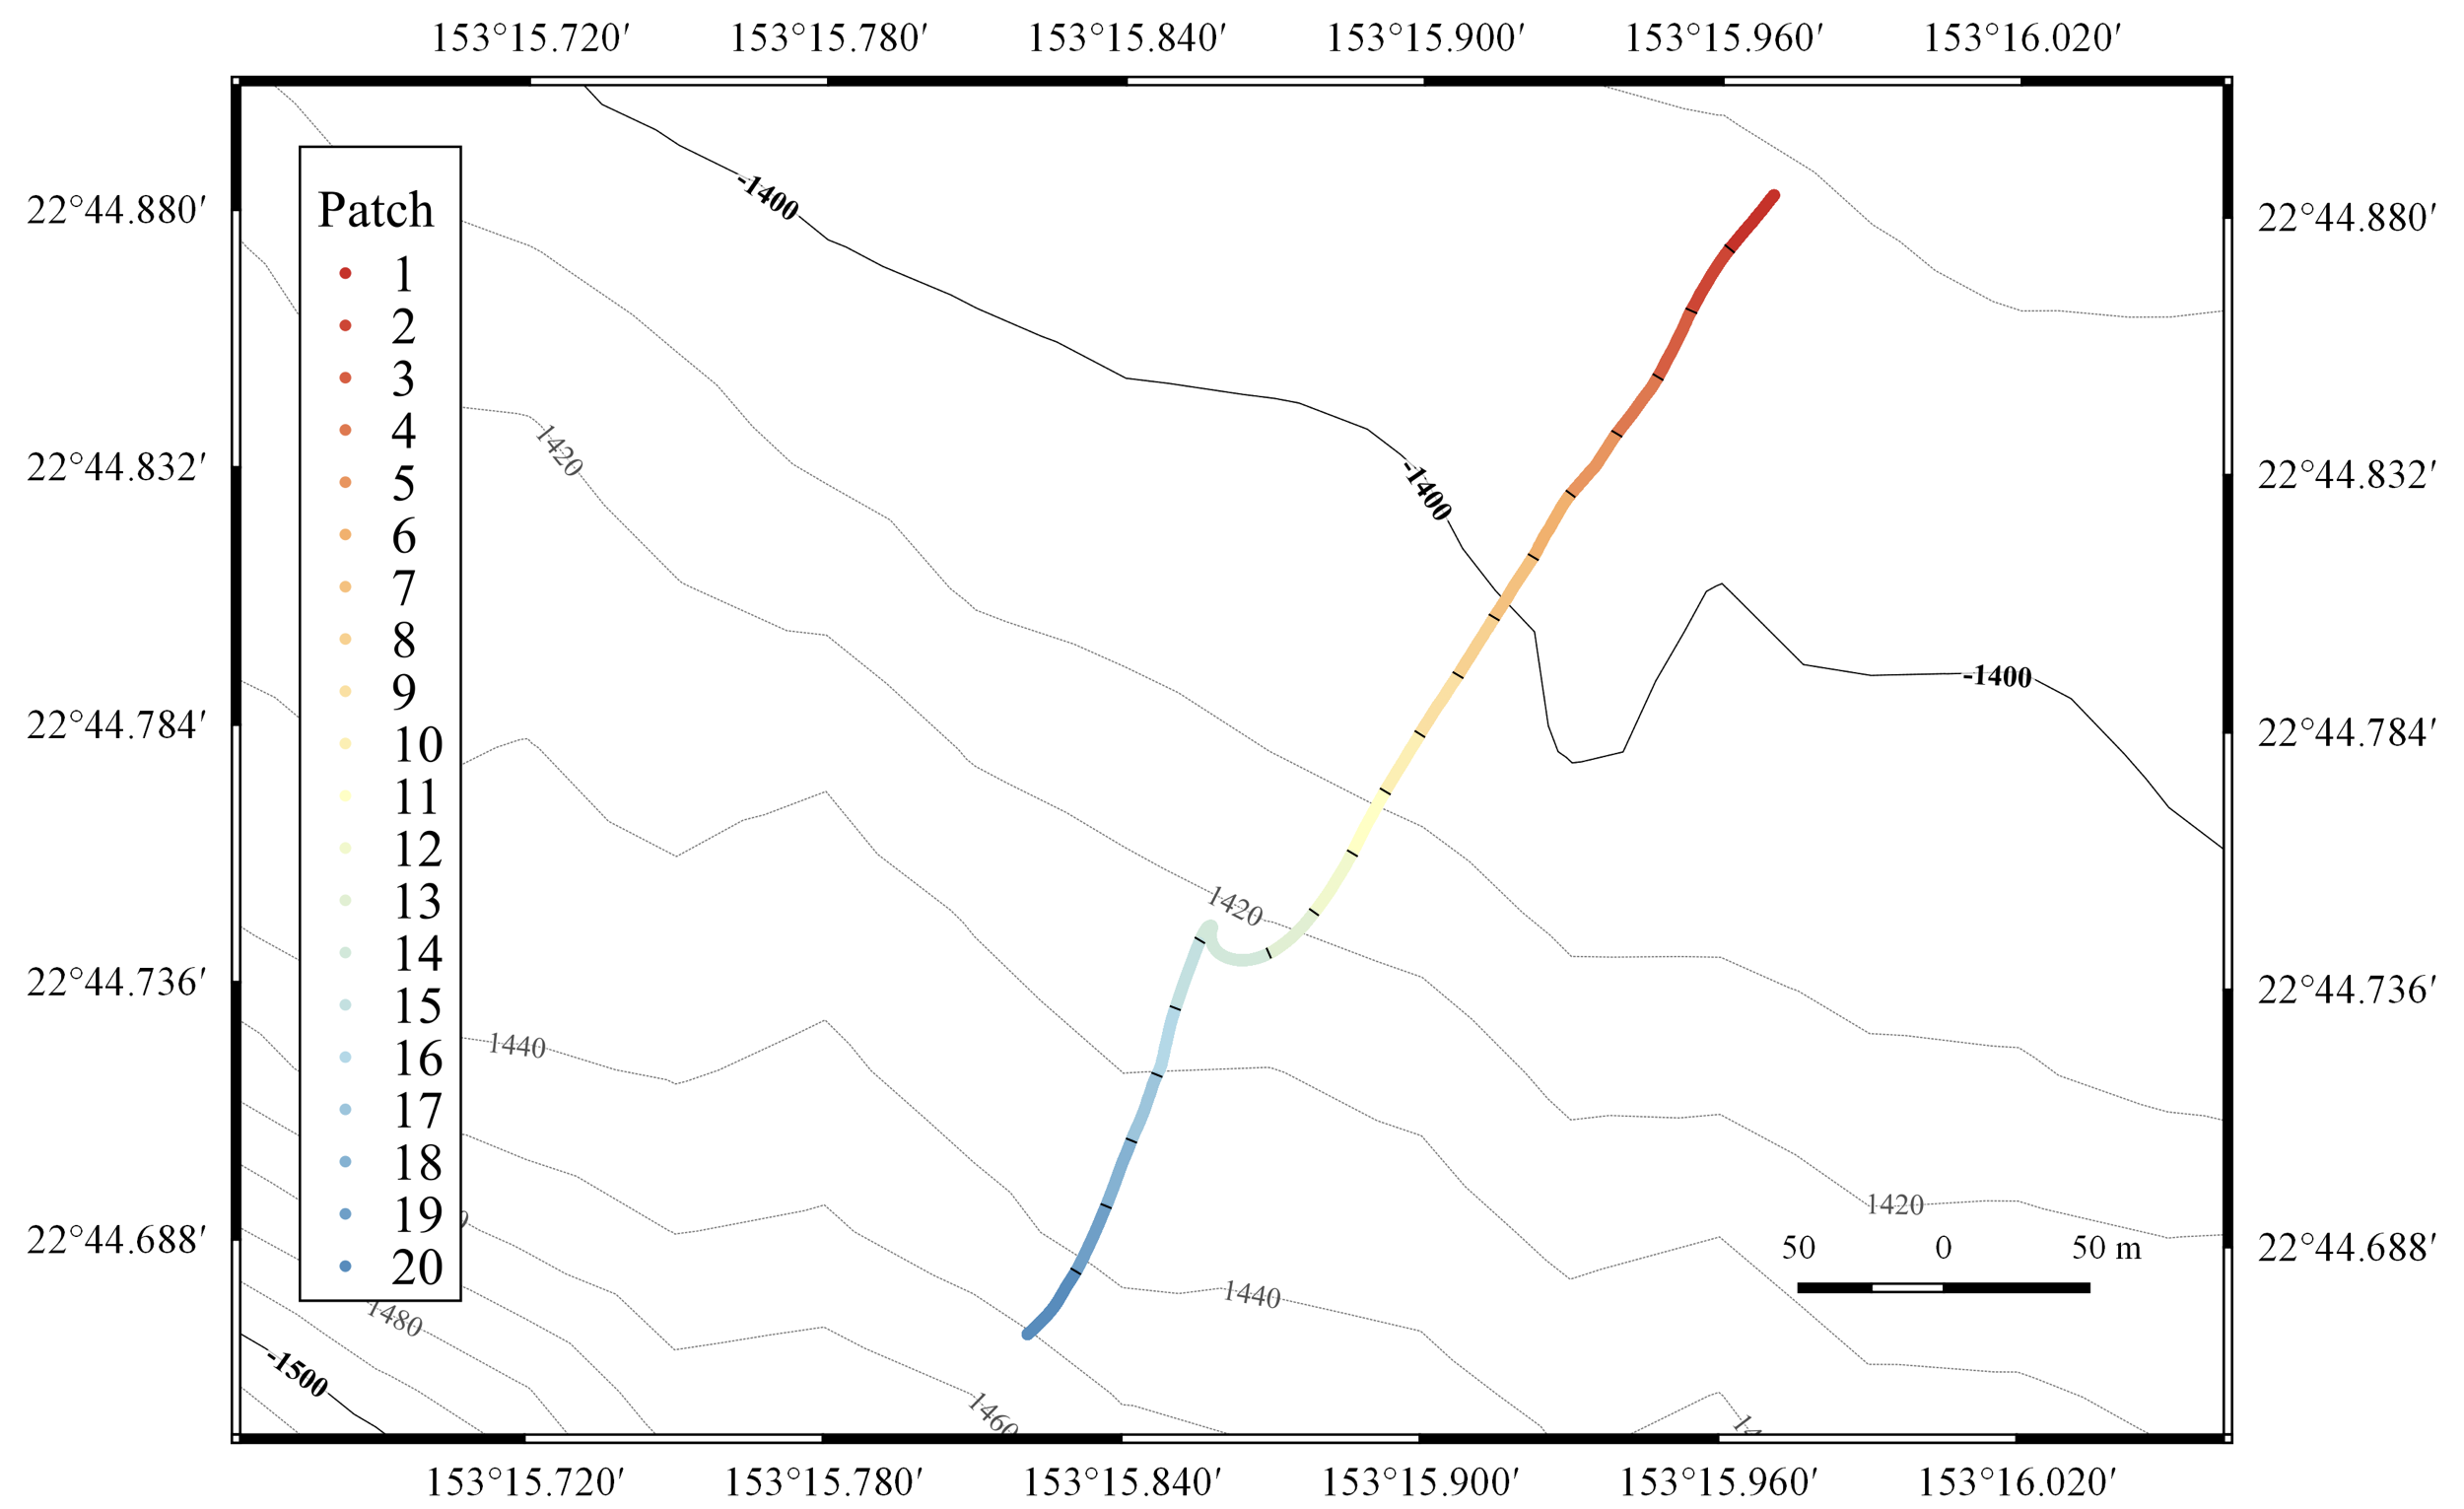
\includegraphics[width=6in]{./images/mehul24.png}
\caption{Vehicle trajectory at No.$5$ Takuyo seamount where the algorithm is implemented on $20$ patches}
\label{f:mehul24}
\end{figure}

The northern part of the seamount has a more gentle 
	slope while the lower regions contain rocky and pillowy outcrops. The number 
	of patches for which the algorithm can successfully detect landing sites is 
	evaluated. The landing cost is analyzed for its relation to the type of 
	seafloor terrain.
	
	
\subsection{Data analysis and results}

The algorithm was implemented on each patch to detect landing sites and select a final landing site and heading. The dimensions of the underwater vehicle were kept identical to those used for simulation in Section ~\ref{sec:algo}, as mentioned in Table~\ref{t:table2}. The other parameters for the landing algorithm are identical since the vehicle dimensions used are the same. The algorithm was able to detect a landing site in each patch the properties of which can be seen in Fig~\ref{sf:mehul25}. The landing heading for each patch is close to the mapping heading due to the narrow swath of the bathymetry as in Fig~\ref{sf:mehul26}.

\begin{figure}[!ht]
\centering
\subfloat[Final landing site properties and landing cost for all patches\label{sf:mehul25}]{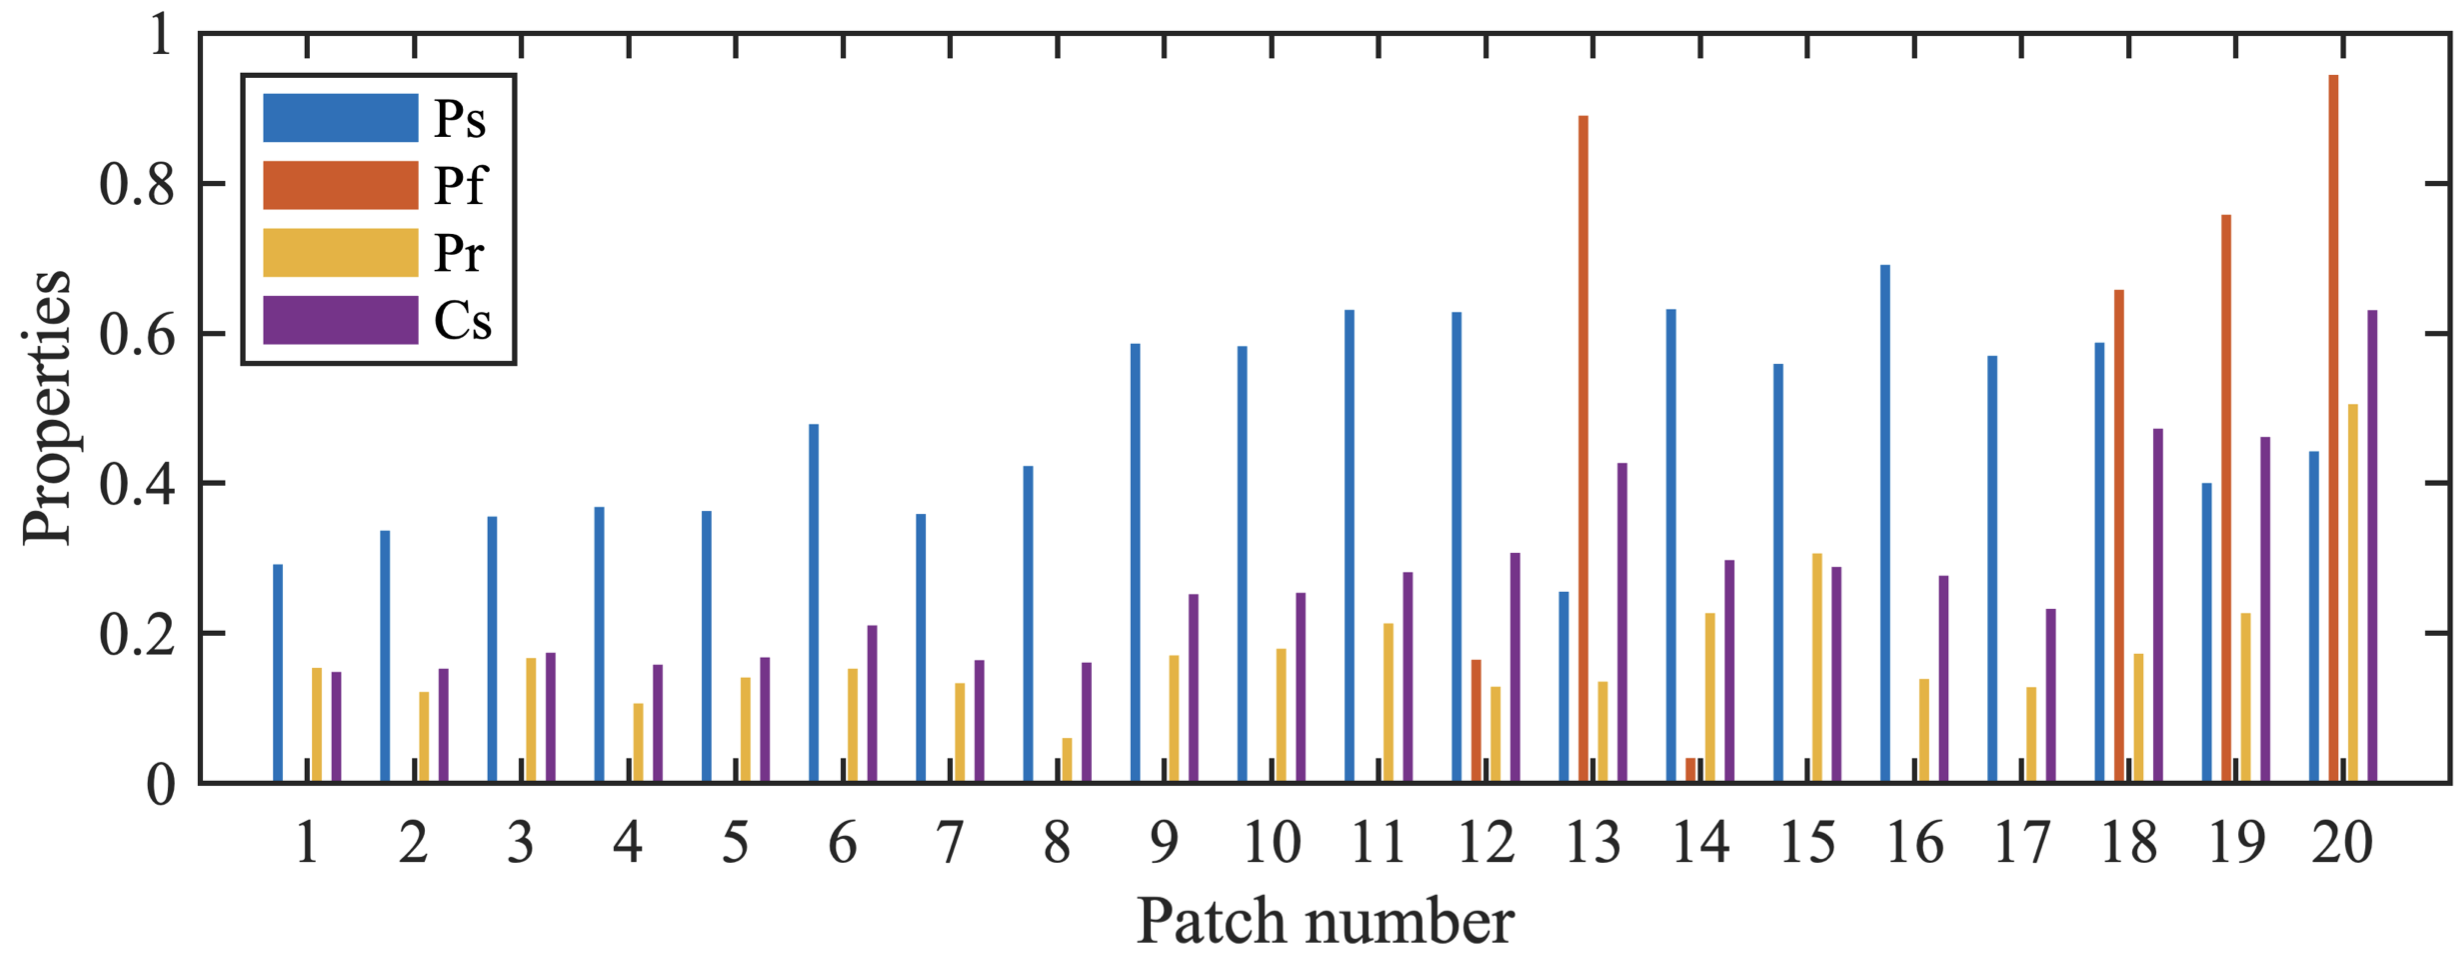
\includegraphics[width=5.5in]{./images/mehul25.png}}\quad
\subfloat[Final landing site headings for all patches\label{sf:mehul26}]{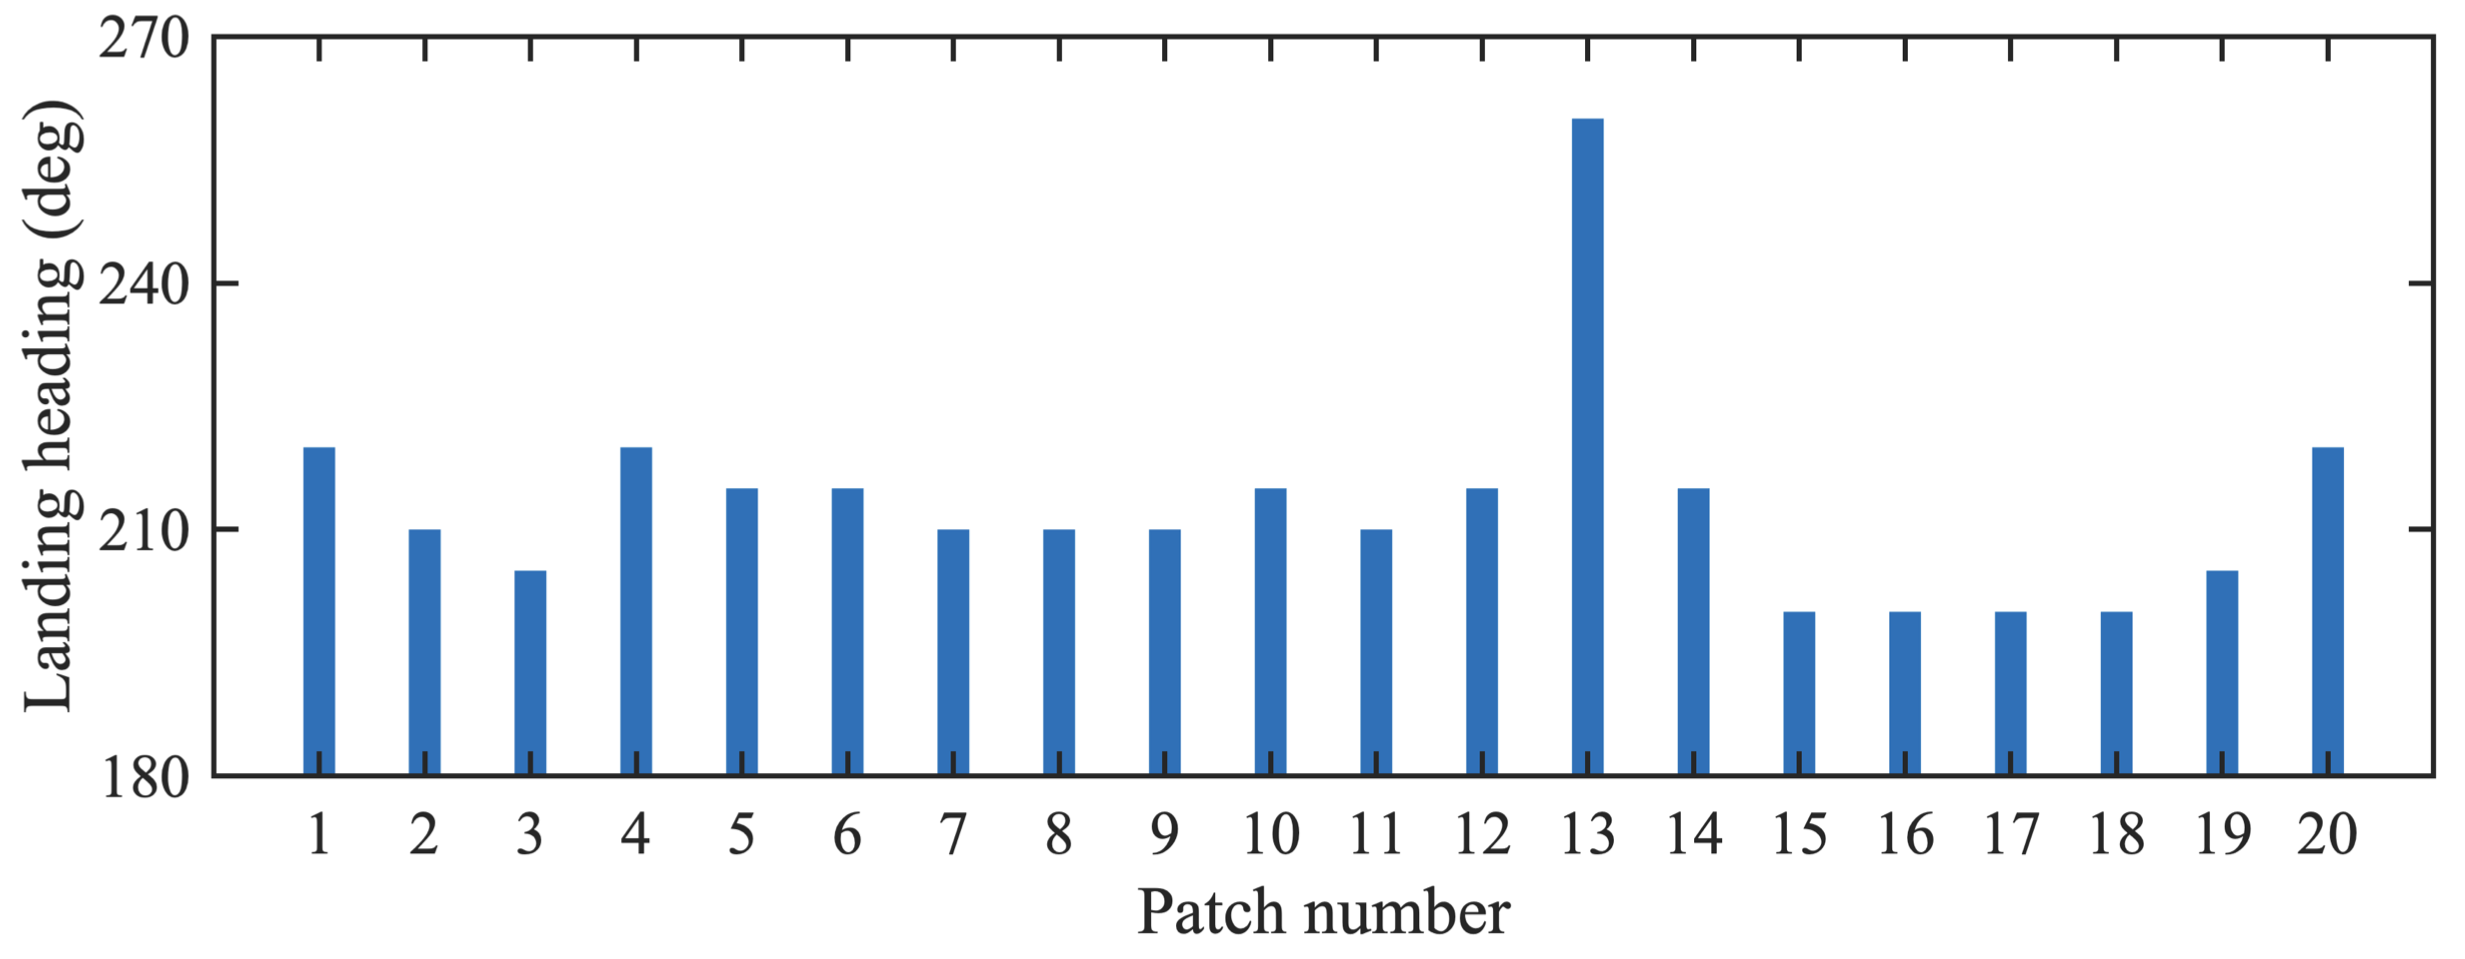
\includegraphics[width=5.5in]{./images/mehul26.png}}
\caption{Results of implementation of landing algorithm on all patches}
\end{figure}

The landing costs for sites towards the south of the transect show higher values due to the rough and steep sloping nature of the seafloor as see in Fig~\ref{f:mehul27}. The mean Cs value is found to be $0.27$. All the sites show high values for Ps due since the mapped bathymetry is along the slope of the seamount. Fig~\ref{f:mehul28} shows the final landing sites for three patches along different locations in the transect. Patch $1$ has the least landing cost due to the wide swath, gently sloping smooth surface. Patch $2$ shows narrow landing area due to reduced mapping swatch while turning but is smooth and gently sloping. Patch $3$ towards he lower end of the transect shows extremely narrow landing area, rough surface with high slope thereby making the highest landing cost.

\begin{figure}[!ht]
\centering
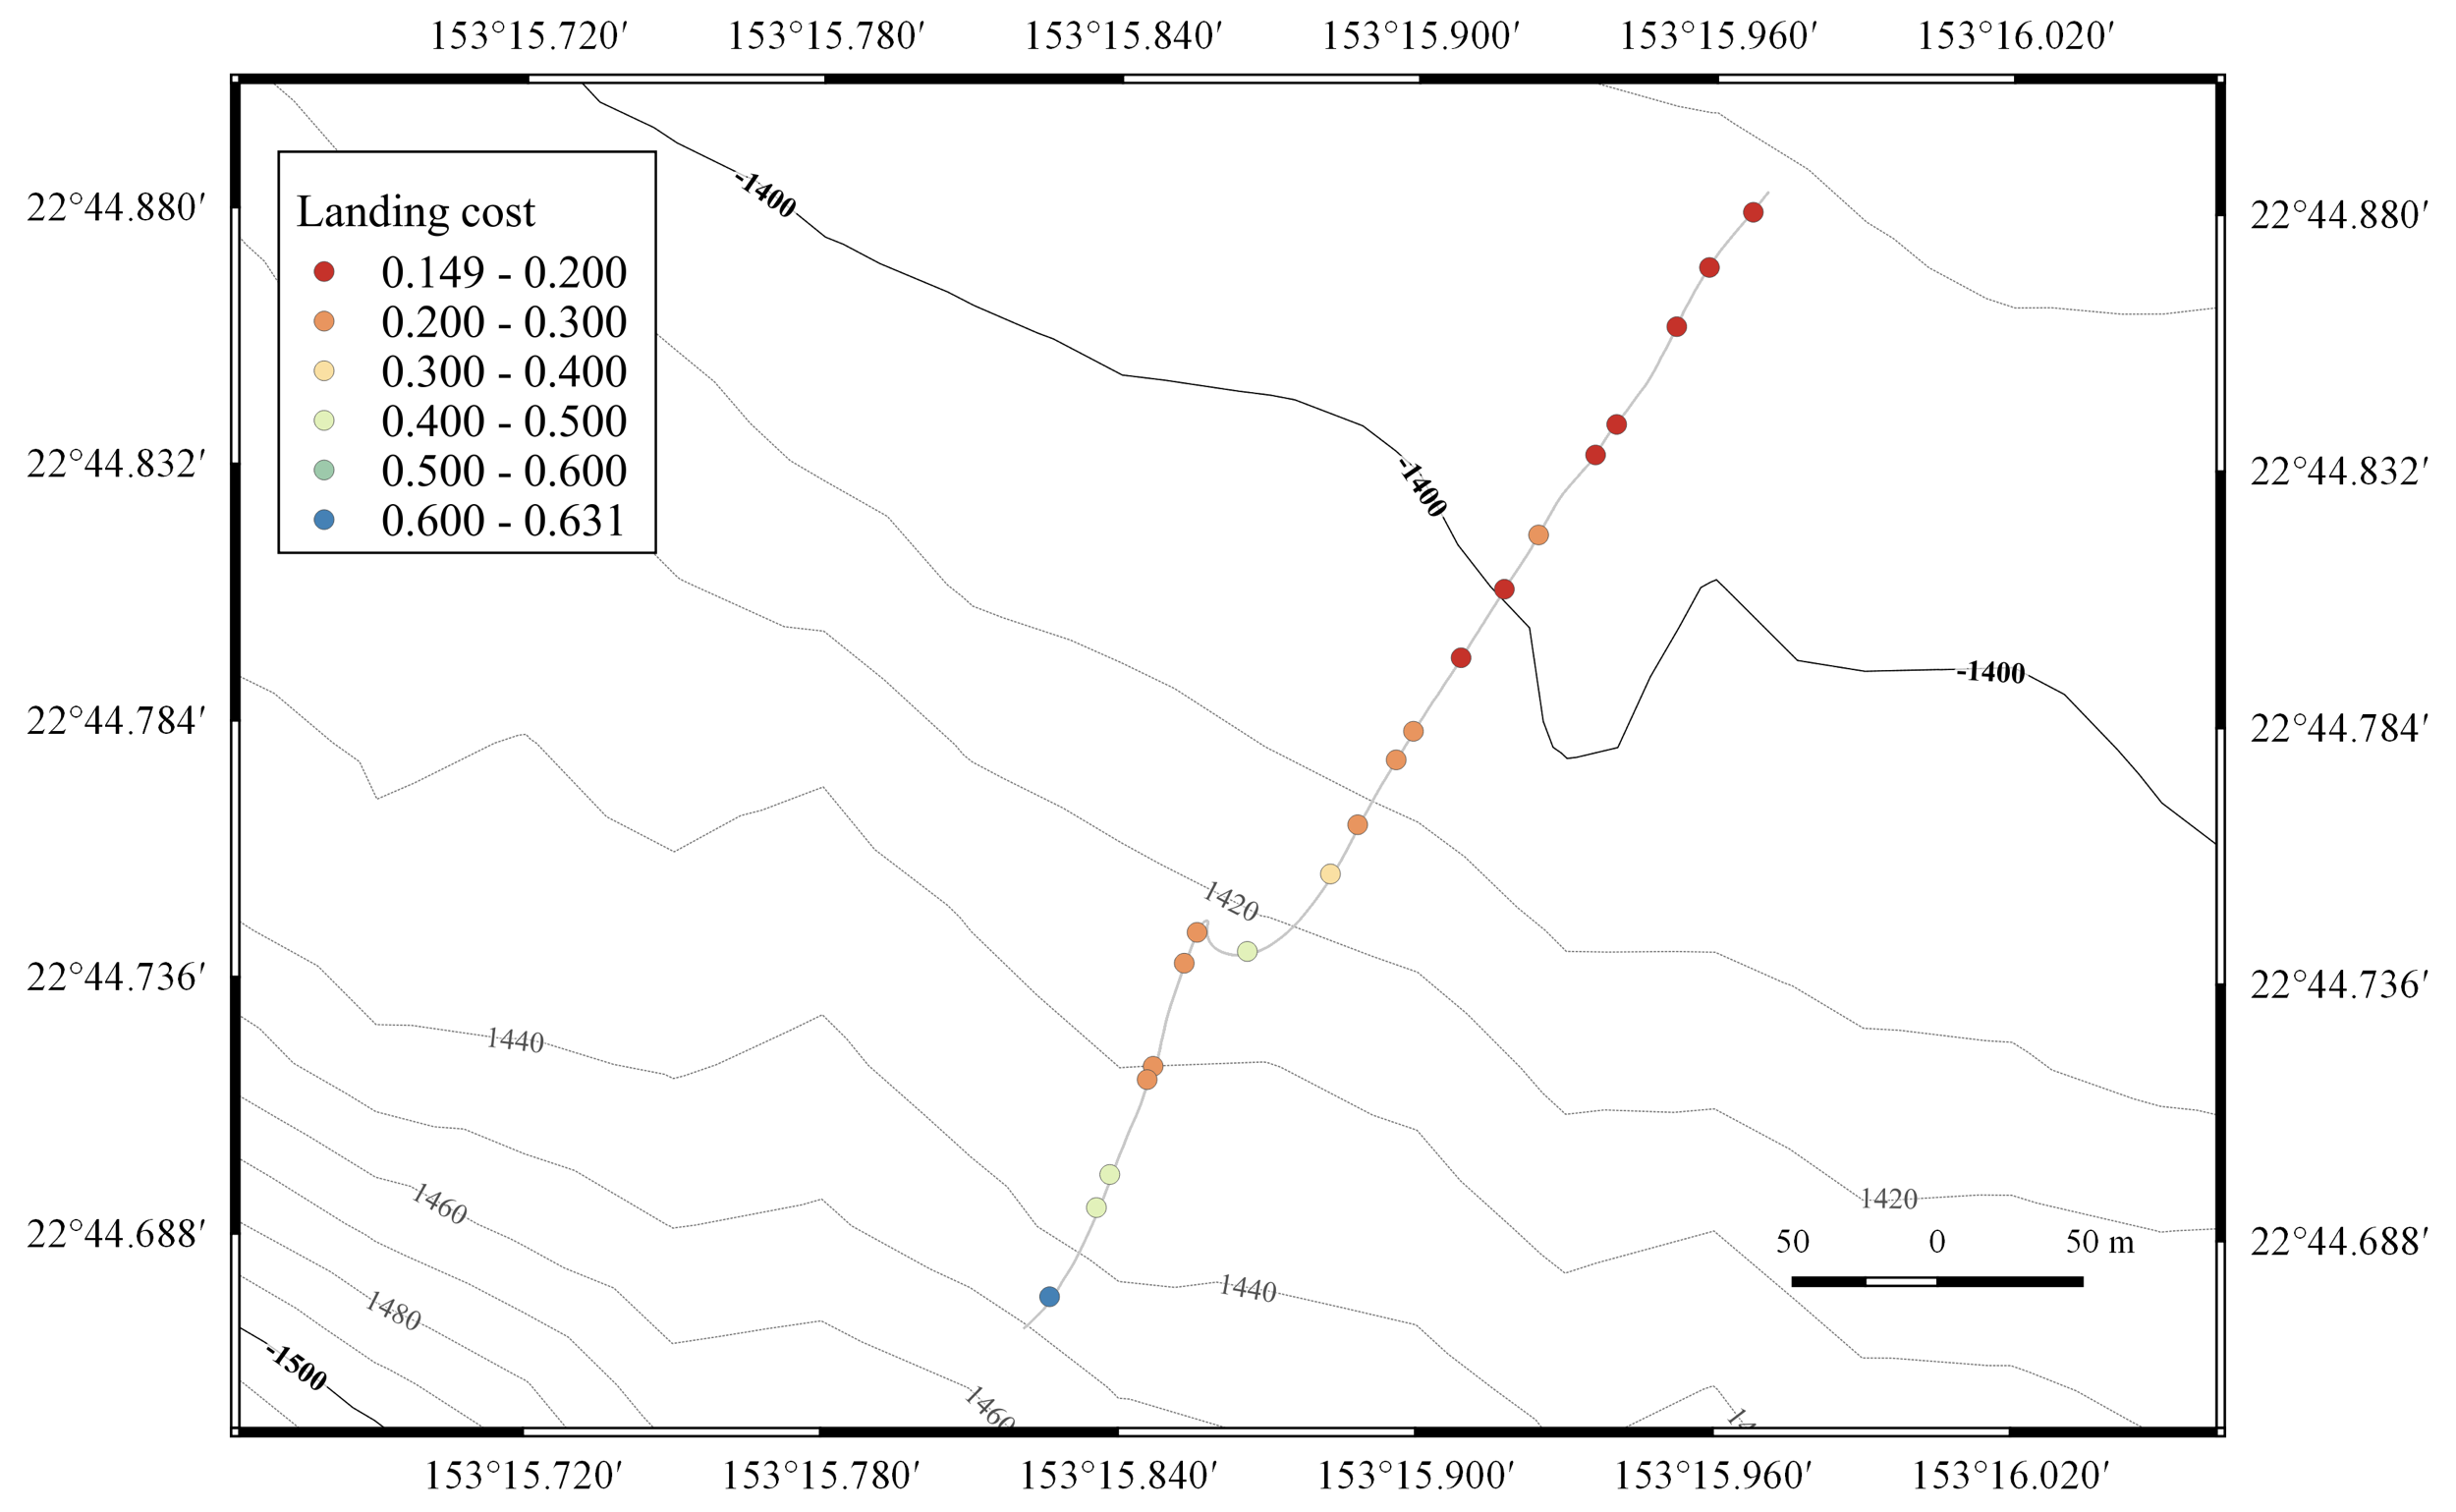
\includegraphics[width=6in]{./images/mehul27.png}
\caption{Landing cost for sites identified}
\label{f:mehul27}
\end{figure}


\begin{figure}[!ht]
\centering
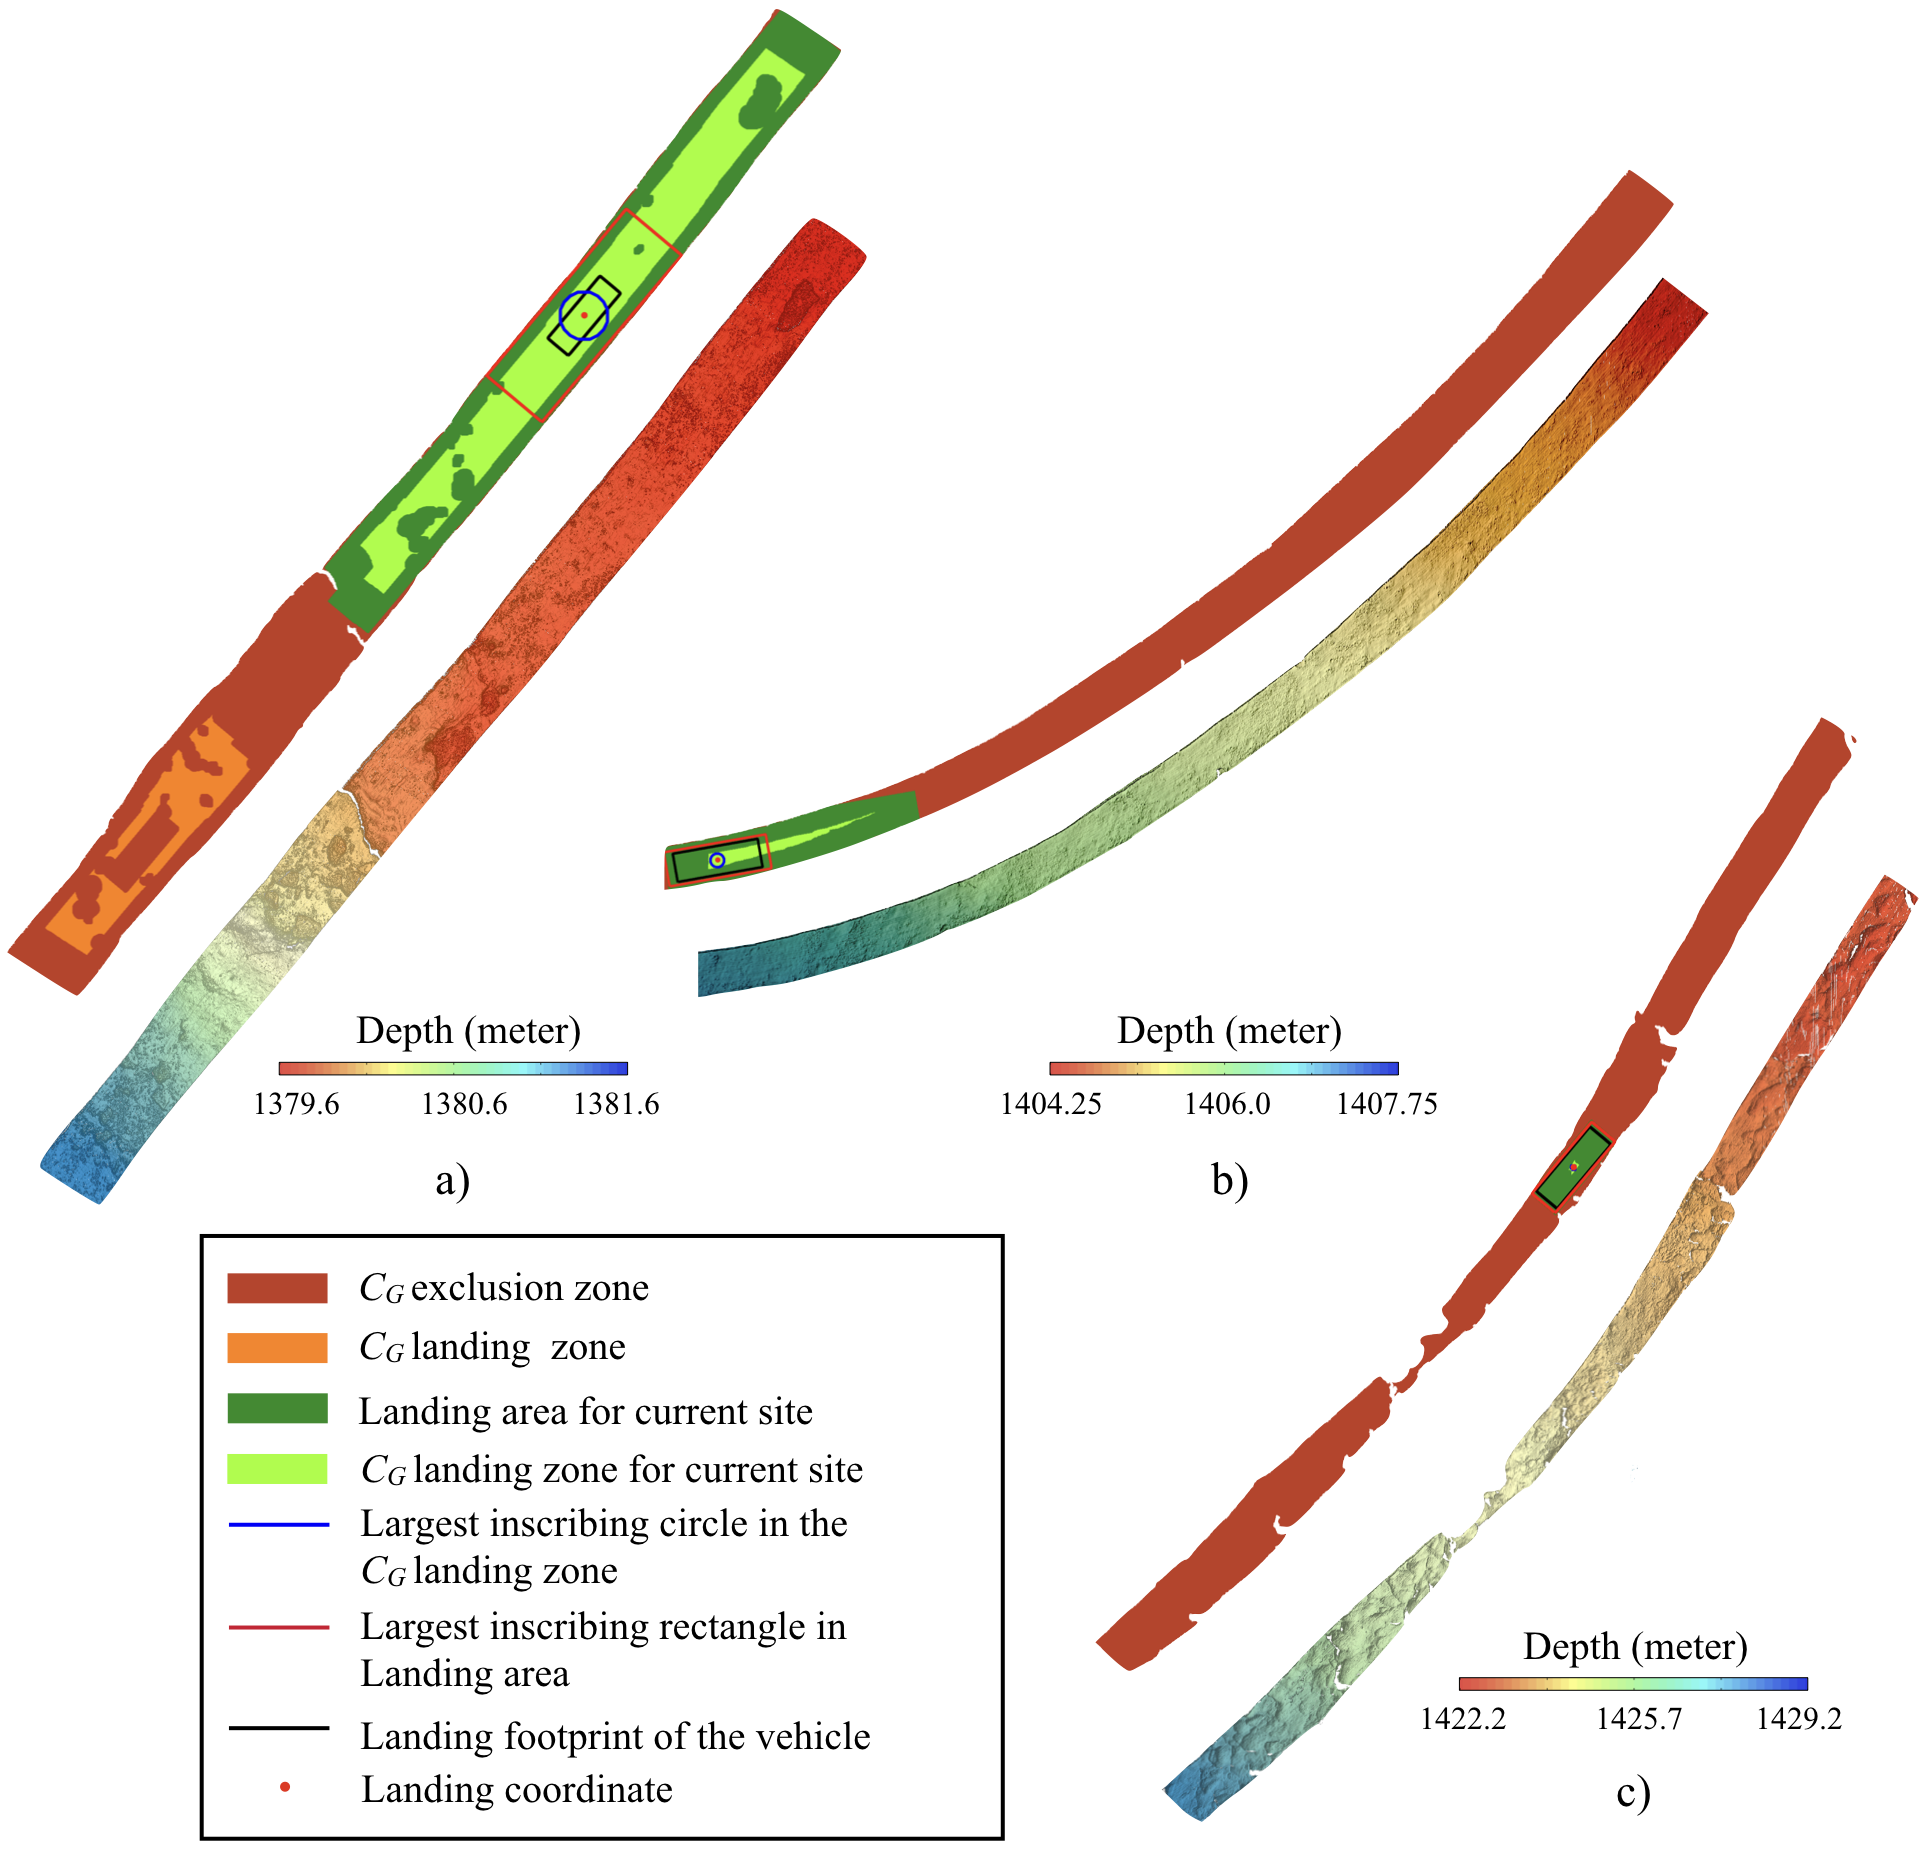
\includegraphics[width=\textwidth]{./images/mehul28.png}
\caption{Landing cost for sites identified}
\label{f:mehul28}
\end{figure}

\begin{table}[!ht]
\centering
\caption{Results of analysis on mapped bathymetry}
\begin{tabular}{  |c c c c c|}
\hline
\textbf{Area surveyed} & \textbf{Number of sites} & \textbf{Mean landing cost} & \textbf{Landing cost range} & \textbf{Landing cost Std. Dev.}\\ \hline 
$794.4$ sq.m. & $754$ & $0.28$ & $0.15 - 0.63$ & $0.13$ \\
\hline
\end{tabular}
\label{t:table6}
\end{table}
